\chapter{ဒေတာဘေ့စ်များနှင့် ဆက်သွယ်ဆောင်ရွက်ခြင်း}

ဒေတာဘေ့စ်တွေဟာ ကနေ့ခေတ် \fEn{information system} အားလုံးရဲ့ အဓိကကျောရိုးလို့ ဆိုနိုင်ပါတယ်။ ၎င်းတို့ဟာ \fEn{web application} တွေမှာ အသုံးပြုသူ ကိုယ်ရေးအချက်အလက်ကနေ ဘဏ္ဍာရေးဆိုင်ရာ အဖွဲ့အစည်းကြီးတွေ ငွေဝင်ငွေထွက် စာရင်းအထိ အရာအားလုံး သိမ်းဆည်းပေးတဲ့ စနစ်တွေ ဖြစ်တယ်။ ကျန်းမာရေး၊ စီးပွားရေး၊ ပညာရေး၊ ဘဏ္ဍာရေး စတဲ့ ကဏ္ဍ အားလုံးမှာ အချက်အလက်တွေ ထိထိရောက်ရောက် သိမ်းဆည်း စီမံနိုင်ဖို့အတွက် ဒေတာဘေ့စ်တွေက မရှိမဖြစ်ပါပဲ။ အရေးပါတဲ့ ဒီလို ကဏ္ဍတွေမှာ လုပ်\allowbreak ငန်းအသီးသီး မှန်ကန်တိကျ၊ နောက်ဆုံးရ အချက်အလက်တွေနဲ့  \fEn{informed decision} ချနိုင်ဖို့ အဓိကဆောင်ရွက်ပေးတဲ့ စနစ်တွေလည်း ဖြစ်တယ်။

ဒီအခန်းမှာ \fEn{Python} နဲ့ ဒေတာဘေ့စ် ချိတ်ဆက်အသုံးပြုပုံကို လေ့လာကြမှာပါ။ အခြေ\allowbreak ခံ ဒေတာဘေ့စ် \fEn{concept} တွေကိုတော့ ဒီစာအုပ်မှာ အကျဉ်းချုံးလောက်ပဲ ဖော်ပြပေးနိုင်မယ်။ ပရော်ဖက်ရှင်နယ် အဆင့် ဒေတာဘေ့စ် ပရိုဂရမ်းမင်း အတွက်ဆိုရင် တချို့အပိုင်းတွေကို ထဲထဲဝင်ဝင် ဆက်လက် လေ့လာရပါလိမ့်မယ်။ ကိုးကားစာအုပ်တွေ နောက်ဆုံးမှာ ကြည့်နိုင်ပါတယ်။

% \fEn{Databases are the backbone of modern information systems. They store everything from user data in web applications to transaction records in financial systems. They are used in virtually every industry, including finance, healthcare, e-commerce, and education, to store and manage data efficiently, enabling businesses to make informed decisions based on accurate and up-to-date information.}

\section{Database Management Systems}
‘ဒေတာဘေ့စ်’ ဆိုတာ အချက်အလက် အမြောက်အများ ရေရှည်သိမ်းဆည်းပေးတဲ့ စနစ်လို့ အကြမ်းဖျဉ်း ပြောနိုင်ပါတယ်။ သာမန်အားဖြင့် ရေရှည်သိမ်းထားချင်ရင် ဖိုင်စနစ် သုံးလို့ရပေမဲ့ ဒေတာ များလာတဲ့အခါ အဆင်မပြေနိုင်တော့ဘူး။ ပြန်လည်ရှာဖွေရတာ၊ ထုတ်ယူရတာ၊ အမြဲတမ်း မှန်ကန်ကိုက်ညီနေအောင် ထိန်းသိမ်းရတဲ့ ကိစ္စတွေအတွက် ပြဿနာရှိလာတယ်။ \fEn{Database Management Systems (DBMS)} တွေကို ဒီအခက်အခဲတွေ ဖြေရှင်းပေးဖို့  တီထွင်ခဲ့ကြတာပါ။ အချက်အလက် မှန်ကန်တိကျခြင်း၊ လုံခြုံမှုရှိခြင်းနှင့် အလွယ်တကူ \fEn{access} လုပ်နိုင်ခြင်းအတွက် \fEn{DBMS} တွေမှာ ဦးစားပေး ထည့်သွင်း စဉ်းစားထားတယ်။ ဒေတာပမာဏ အများအပြား စနစ်တကျ ထိထိရောက်ရောက် စုဆောင်း၊ သိမ်းဆည်း၊ စီမံဖို့အတွက် အားကိုးအားထားပြုရတဲ့ စနစ်တွေလို့ ဆိုရမယ်။  

\subsection*{သမိုင်းအကျဉ်း}
ဒေတာဘေ့စ်တွေရဲ့ မူလအစ \fEn{concept} ဟာ \fEn{IBM} ကုမ္ပဏီက \fEn{IMS (Information Management System)} လို စနစ်တွေ တည်ဆောက်ခဲ့တဲ့ ၁၉၆၀ ခုနှစ်တွေလောက်ကို ပြန်သွားနိုင်တယ်။ အဲ့ဒီစနစ်တွေက \fEn{hierarchical} ဖြစ်တယ်။ ဆိုလိုတာက ဒေတာသိမ်းတဲ့ စထရက်ချာက သစ်ပစ်လိုပဲ၊ အပင်ရဲ့ အမြစ်၊ အရွက်၊ အကိုင်းအခက်တွေ ဆက်စပ်နေသလိုပုံစံနဲ့ အချက်အလက်တွေကို သိမ်းတယ်။ \fEn{Parent-child relationship} နဲ့ သိမ်းတာလို့လည်း ဆိုနိုင်တယ်။ ၁၉၇၀ ခုနှစ်တွေမှာတော့ \fEn{Edgar F. Codd} က ယနေ့ခေတ် \fEn{Relational Database Management System (RDBMS)} ရဲ့ အခြေခံအုတ်မြစ် ဖြစ်လာတဲ့ \fEn{Relational Data Model} ကို စတင်မိတ်ဆက်ခဲ့တယ်။ \fEn{Relational model} မှာက ဒေတာသိုလှောင်သိမ်းဆည်းဖို့ \fEn{table} တွေကို အသုံးပြုပြီး \fEn{SQL (Structured Query Language)} လို့ခေါ်တဲ့ \fEn{programming language} ကို ထောက်ပံပေးပါတယ်။ 

\subsection*{SQL Language}
\fEn{SQL} ဟာ  \fEn{table} ဒေတာ အမြောက်အများကနေ မိမိစူးစမ်းလိုတဲ့ အချက်အလက်ကို အလွယ်တကူ ထုတ်ယူ (သို့) မေးမြန်းလို့ရအောင် ကူညီထောက်ပံပေးဖို့ အဓိကရည်ရွယ်တယ်။ “ကေသီ ဒီနှစ် ဇွန်လစာမေးပွဲမှာ ဘာသာရပ်အသီးသီး ရမှတ်ဘယ်လောက်လဲ” လို  ခပ်ရိုးရိုး မေးခွန်းကနေ “ဘယ်ကျောင်းသူ ကျောင်းသား တွေ စာမေးပွဲအားလုံးမှာ သင်္ချာရမှတ် ၉၅ မှတ်အထက် သုံးနှစ်ဆက်တိုက် ရကြလဲ” ဆိုတဲ့ အတော်လေး ရှုပ်ထွေးတဲ့  \fEn{query} မျိုးတွေထိ မြန်ဆန်ထိရောက်စွာ လုပ်ဆောင်ပေးနိုင်ပါတယ်။ 

အချက်အလက် ထုတ်ယူတာအပြင် ဒေတာဘေ့စ် အသစ်ဆောက်တာ၊ \fEn{table} ဆောက်တာ၊ ပြန်ဖျက်တာ စတဲ့ကိစ္စတွေကိုလည်း \fEn{SQL} နဲ့ပဲ လုပ်ရပါတယ်။ \fEn{Table} မှာ \fEn{record} အသစ်ထည့်တာ၊ ရှိပြီးသား \fEn{record} ကို \fEn{update} လုပ်တာ၊ ဖျက်ပစ်တာ စတာတွေအတွက်လည်း \fEn{SQL} ကိုပဲ သုံးရတာပါ။ 

\fEn{SQL} ဟာ \fEn{RDBMS} အားလုံးမှာ အသုံးပြုနိုင်တဲ့ \fEn{standard language} တစ်ခုလည်းဖြစ်တယ်။ ဆိုလိုတာက ဘယ် \fEn{RDBMS} ကိုပဲ သုံးသုံး၊ \fEn{SQL} တစ်မျိုးတည်းကိုပဲ သုံးရမှာပါ။ \fEn{RDBMS} တစ်ခုမှာ သူ့ကိုယ်ပိုင် ချဲ့ထွင်ထားတဲ့ အပိုင်းတွေ အနည်းအကျဉ်း ရှိကြပေမဲ့ \fEn{SQL standard} ကို ရာနှုန်းပြည့် မဟုတ်တောင် အဲ့လောက်နီးနီး လိုက်နာထားကြတဲ့အတွက် ပြောပလောက်အောင် မကွာကြဘူး။ \fEn{SQL} သာနားလည်ပါစေ၊ ဘယ်ဒေတာဘေ့စ်နဲ့မဆို အလုပ်ဖြစ်တယ်လို့ ပြောရင်လည်း မမှားဘူး။

\subsection*{Client-Server Applications}
တစ်ချိန်မှာ တစ်ယောက်ပဲ သုံးလို့ရတဲ့ ဆော့ဖ်ဝဲတွေနဲ့ မတူတာက \fEn{DBMS} တွေဟာ တစ်ယောက်မက တပြိုင်နက် သုံးလို့ရတဲ့ ဆာဗာ \fEn{(server)} ဆော့ဖ်ဝဲတွေ ဖြစ်ပါတယ်။ တပြိုင်နက် ဝင်ရောက်လာတဲ့ အသုံးပြုသူတွေရဲ့ တောင်းဆိုချက်တွေကို ဖြည့်ဆည်းဖို့အတွက် ကိုင်တွယ်ဆောင်ရွက် ပေးနိုင်စွမ်း ရှိတယ်။ 

တစ်ခုထက်ပိုတဲ့ \fEn{client} တွေက ဆာဗာတစ်ခုနဲ့ ချိတ်ဆက်အသုံးပြုတဲ့ ဆော့ဖ်ဝဲစနစ်မျိုးကို  \fEn{Client-Server Application} လို့ ခေါ်တယ်။ \fEn{Client} ဆိုတာ အသုံးပြုသူ \fEn{user} (သို့) ၎င်းအသုံးပြုတဲ့ ပရိုဂရမ်ကို ဆိုလိုတာ။ ဒေတာဘေ့စ် \fEn{application} အများစုဟာ \fEn{Client-Server Application} တွေပါ။ \fEn{Web Application} တွေဟာ \fEn{Client-Server Application} ဖြစ်ပြီး ဒေတာသိမ်းဖို့အတွက် နောက်ကွယ်က \fEn{RDBMS} တစ်ခုနဲ့ ချိတ်ဆက်ထားရလေ့ရှိတယ်။ 


\section{PostgreSQL}
ဒီစာအုပ်မှာ \fEn{PostgreSQL RDBMS} အသုံးပြုပါမယ်။ \fEn{PostgreSQL} ဘယ်လို အင်စတောလ်လုပ်မလဲ စာမျက်နှာ \fRefNo{\pageref{apdx3}} နောက်ဆက်တွဲ (\fRefNo{\ref{apdx3}}) မှာ ကြည့်ပါ။ \fEn{psql} ဖွင့်ပြီး \fEn{root user (postgres)} အနေနဲ့ \fEn{PostgreSQL} ဒေတာဘေ့စ်ကို ချိတ်ဆက်ထားပါ။

\subsection*{ဒေတာဘေ့စ် အသစ်ဆောက်ခြင်း}
ဒေတာဘေ့စ် အသစ်တစ်ခု ဆောက်မယ်ဆိုရင် \fCode{CREATE DATABASE} \fEn{SQL} ကွန်မန်း သုံးပါတယ်။  
%
\begin{sql}
CREATE DATABASE ß\fEnEmp{database\_name}ß;
\end{sql}
%
\fEn{SQL language} ဟာ စာလုံး အကြီးအသေး မခွဲဘူး။ ဒီစာအုပ်မှာ \fEn{SQL keyword} တွေဆိုရင် အက္ခရာအကြီးနဲ့ ရေးပါမယ်။ \fEn{Database, table, column, function} စတာတွေရဲ့ နံမည်တွေက အက္ခရာအသေးနဲ့ ဖြစ်မယ်။
\fEn{student} ဒေတာဘေ့စ် အတွက် ဒီ \fEn{SQL} ကို
%
\begin{sql}
CREATE DATABASE students;
\end{sql}
%
\fEn{psql} ကနေ \fEn{run} ပေးပါ $\big\llbracket$ပုံ (\fRefNo{\ref{fig:createdb}})$\big\rrbracket$။ \fEn{SQL} စတိတ်မန့် တစ်ကြောင်း အဆုံးမှာ ဆီမီးကော်လံ \fEn{(\fCode{;})} ထည့်ပေးရပါမယ်။

\begin{figure}[tb!]
\begin{tikzpicture}
    \node[anchor=south west,inner sep=0] (image) at (0,0)
    {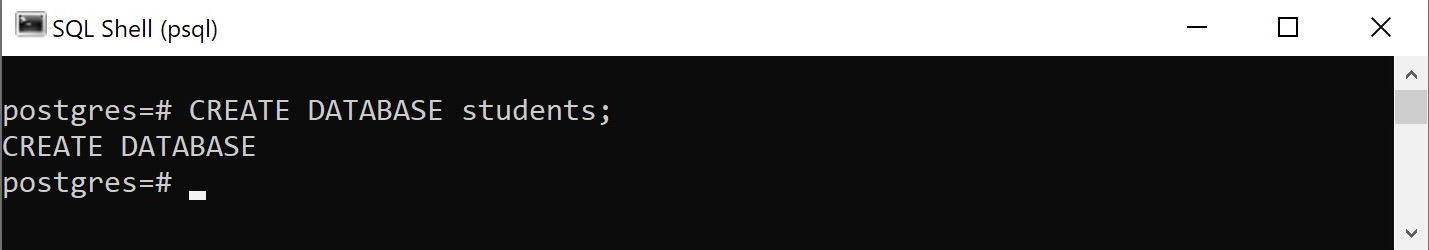
\includegraphics[width=.98\linewidth, trim={0mm, 0.5mm, 0.5mm, 0.5mm}, clip]{images/ch12/createdb.jpg}};
    \drawshadow{image}
\end{tikzpicture}
\caption{}
\label{fig:createdb}
\end{figure}

\fEn{psql} ကနေ \mintinline{text}|\l| (သို့) \mintinline{text}|\list| ကွန်မန်းနဲ့ \fEn{PostgreSQL} မှာ ရှိတဲ့ ဒေတာဘေ့စ်တွေကို ထုတ်ကြည့်နိုင်ပါတယ်။ \mintinline{text}|\l| က \fEn{SQL} မဟုတ်ဘူး။ \fEn{psql} သီးသန့် ကွန်းမန်းတစ်ခုဖြစ်တာကြောင့် ဒီကွန်မန်းကို \fCode{;} မထည့်ဘဲ \fEn{run} ရပါမယ်။ \mintinline{text}|\l| \fEn{run} လိုက်ရင် စာရင်းထဲမှာ \fEn{students} ဒေတာဘေ့စ် တွေ့ရမှာပါ $\big\llbracket$ပုံ (\fRefNo{\ref{fig:listdb}})$\big\rrbracket$။

\begin{figure}[tb!]
\begin{tikzpicture}
    \node[anchor=south west,inner sep=0] (image) at (0,0)
    {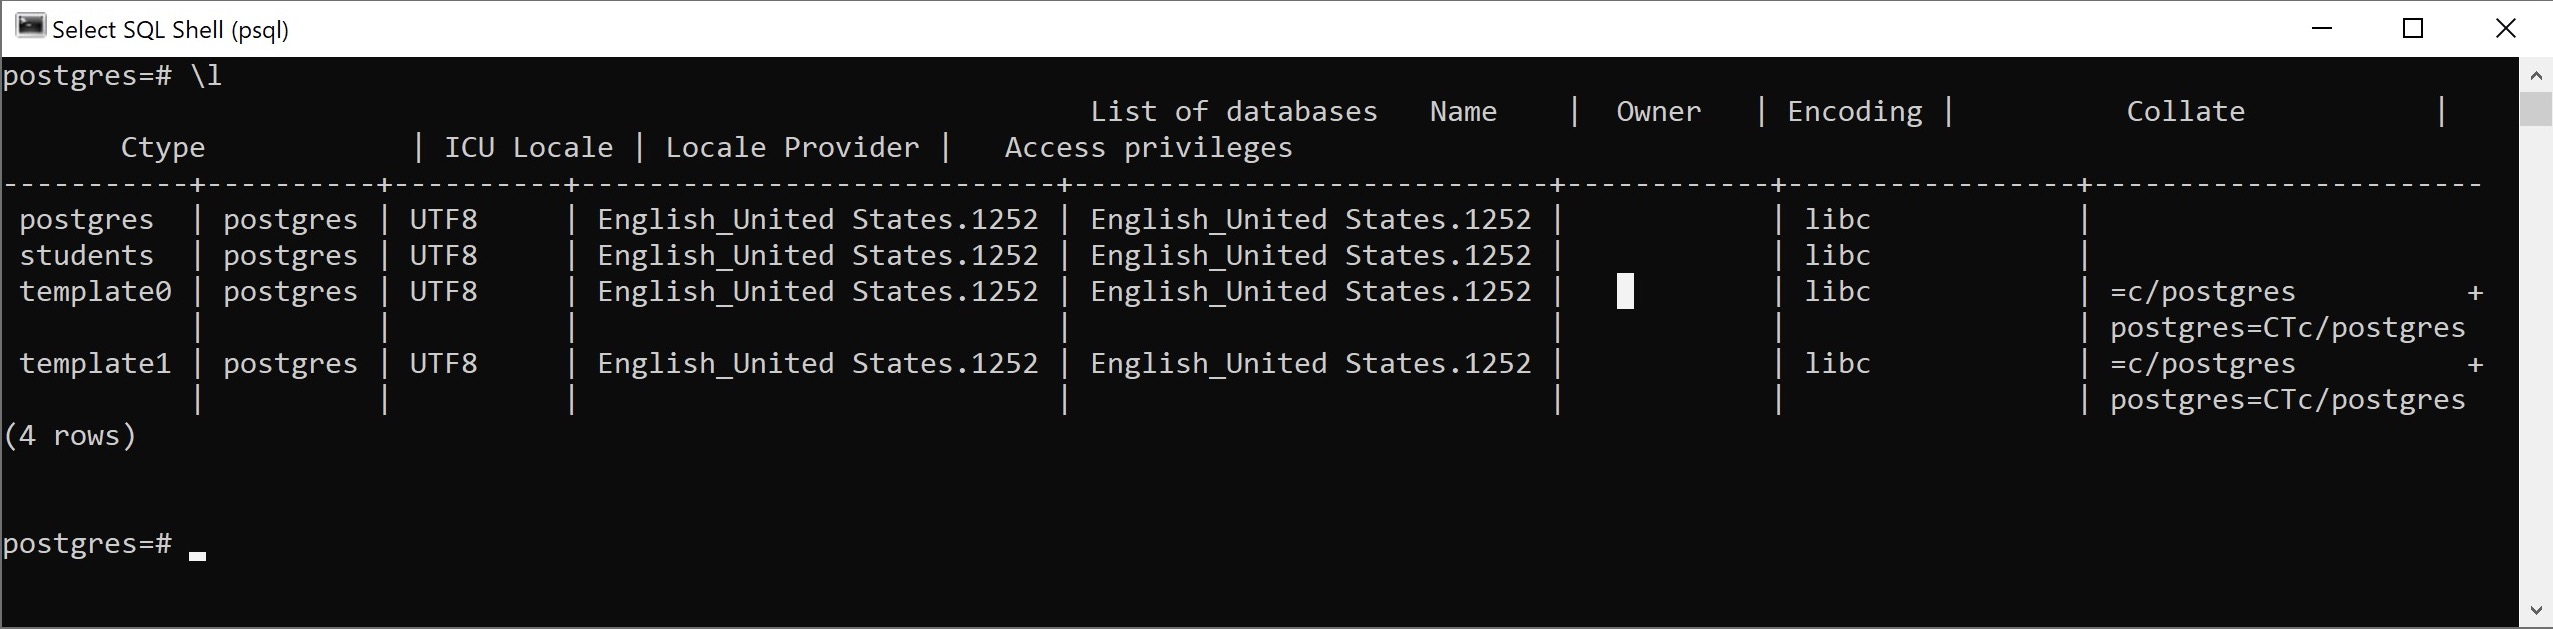
\includegraphics[width=.98\textwidth, trim={0mm 20mm 380mm 0.5mm},clip]{images/ch12/listdb.jpg}};
    \drawshadow{image}
\end{tikzpicture}
\caption{}
\label{fig:listdb}
\end{figure}

\fEn{psql} မှာ ဒေတာဘေ့စ် ပြောင်းချိတ်မယ်ဆိုရင် \mintinline{text}|\c| (သို့) \mintinline{text}|\connect| နဲ့ ပြောင်းရပါမယ်။ \fEn{psql} သီးသန့် ကွန်မန်းပါ။ \fEn{Backslash (}\mintinline{text}|\|\fEn{)} စရင် \fEn{psql} ကွန်းမန်းလို့ မှတ်နိုင်တယ်။ \fEn{students} ဒေတာဘေ့စ်ကို အခုလို \fEn{connect} လုပ်ပါ
\begin{codetxt}
\c students
\end{codetxt}
\fEn{psql} က ဒီလို ပြပါလိမ့်မယ်
\begin{codetxt}
postgres=# \c students
You are now connected to database "students" as user "postgres".
students=#
\end{codetxt}


\subsection*{Table ဆောက်ခြင်း}
\fCode{CREATE TABLE} က \fEn{table} ဆောက်တဲ့ \fEn{SQL} ကွန်မန်းပါ။ \fEn{students} ဒေတာဘေ့စ်ထဲမှာ \fEn{student table} အောက်ပါအတိုင်း ဆောက်ပါမယ်
%
\begin{sql}
CREATE TABLE student (
    id SERIAL PRIMARY KEY,
    name VARCHAR(100),
    age INT,
    grade VARCHAR(2)
);
\end{sql}
%  
\fEn{psql} မှာ \fEn{SQL} \fEn{run} ရင် လက်ရှိချိတ်ထားတဲ့ ဒေတာဘေ့စ်ကို အဲဒီ \fEn{SQL} ပေးပို့ လုပ်ဆောင်ခိုင်းပါတယ်။ အခုချိတ်ထားတာ \fEn{students} ဒေတာဘေ့စ်ဆိုတော့ \fEn{table} ကို အဲဒီ ဒေတာဘေ့စ်ထဲ ဆောက်ပေးသွားမှာပါ။ ဒီ \fEn{table} မှာ \fCode{id}\fEn{,} \fCode{name}\fEn{,} \fCode{age} နဲ့ \fCode{grade} \fEn{column} လေးခုရှိမယ်။

\fEn{Column} တစ်ခုစီမှာ \fEn{data type} ရှိရပါမယ်။ \fCode{VARCHAR(100)} က အများဆုံး ကာရက်တာ အလုံးတစ်ရာ သိမ်းဆည်းနိုင်တယ်။ သိမ်းတဲ့ ကာရက်တာ အရေအတွက်ပေါ် မူတည်ပြီး နေရာယူတာ အနည်းအများ ကွာတယ်။ ငါခုသိမ်းရင် ငါးခုစာ၊ ဆယ်ခုသိမ်းရင် ဆယ်ခုစာပဲ နေရာကုန်မှာပါ။ အမြဲ အလုံး တစ်ရာစာ နေရာကုန်တာ မဟုတ်ဘူး။ \fCode{VARCHAR(2)} ဆိုရင် အများဆုံး  ကာရက်တာ နှစ်လုံး သိမ်းလို့ရမယ်။ \fEn{SQL} \fCode{VARCHAR} က \fEn{Python} \fCode{str} နဲ့ အလားတူတယ်။ \fCode{INT} ကတော့ \fEn{integer} ပါ။

\fCode{id} \fEn{column} က ထူးခြားပြီး နည်းနည်းပိုရှင်းပြဖို့ လိုတယ်။ \fCode{SERIAL} က \fEn{data type} အနေနဲ့ \fCode{INT} နဲ့ တူတူပဲ။ သူ့ရဲ့ ထူးခြားချက်က ဂဏန်းတွေကို အစဉ်အတိုင်း တစ်ခုပြီးတစ်ခု ထုတ်ပေးနိုင်တာပါ။ $1, 2, 3,\ldots$ စသည်ဖြင့်  နောက်ဆုံးတန်ဖိုးကို အလိုအလျောက် တစ်တိုးတိုးပြီး ထုတ်ပေးသွားမှာ ဖြစ်တယ်။ \fCode{id} \fEn{column} က \fEn{Primary Key} လည်းဖြစ်တယ်။ \fEn{Column} တစ်ခုကို \fEn{Primary Key} အဖြစ် ထားချင်ရင် \fCode{PRIMARY KEY} လို့ သတ်မှတ်ရပါမယ်။ \fEn{Primary Key} ဆိုရင် \fEn{column} တန်ဖိုး ထပ် \fEn{(duplicate)} လို့မရဘူး၊ \fEn{unique} ဖြစ်ရပါမယ်။ အခု သိပ်နားမလည်သေးရင်လည်း \fEn{table} မှာ ကျောင်းသား \fEn{record} တွေထည့်တာ ဆက်ကြည့်ရင် ကောင်းကောင်း နားလည်သွားမှာပါ။

\subsection*{\fSubSecCodeBf{INSERT}}
\fEn{Relational Data Model} အခြေခံတဲ့ \fEn{RDBMS} တွေဟာ ဒေတာတွေကို \fEn{table} ပုံစံနဲ့ သိမ်းဆည်းတယ်။ ကျောင်းသူ/သား တစ်ယောက်ချင်းစီအတွက် အချက်အလက်ကို \fEn{student table} မှာ  \fEn{row} တစ်ခုစီနဲ့ ထည့်သွင်း သိမ်းဆည်းပါမယ်။ \fEn{Row} ကို \fEn{record} လို့လည်း သုံးနှုန်းလေ့ရှိတယ်။ \fEn{Record} အသစ် ထည့်သွင်းမယ်ဆိုရင် \fEn{SQL} \fCode{INSERT} ကို သုံးရပါတယ်။

%
\begin{sql}
INSERT INTO student (name, age, grade) VALUES ('Amy', 20, 'A');
INSERT INTO student (name, age, grade) VALUES ('Kathy', 22, 'B');
INSERT INTO student (name, age, grade) VALUES ('Waiyan', 21, 'C');
\end{sql}
%

အေမီ၊ ကေသီ နဲ့ ဝေယံ ကျောင်းသား သုံးယောက်အတွက် \fEn{record} သုံးခု ထည့်သွင်းတာပါ။ \fEn{Column} နံမည်တွေ ဝိုက်ကွင်းထဲမှာ ထည့်ပြီး အဲ့ဒီ \fEn{column} တွေအတွက် တန်ဖိုးအသီးသီးကို အစဉ်အတိုင်း ထည့်ပေးရပါတယ်။ \fCode{age} နဲ့ \fCode{grade} ရှေ့နောက် ဖလှယ်လိုက်မယ်ဆိုရင် အခုလို
%
\begin{sql}
INSERT INTO student (name, grade, age) VALUES ('Amy', 'A',  20);
\end{sql}
%
ဖြစ်ရမှာပါ။

\fEn{student table} မှာ \fEn{column} က လေးခု ရှိတာပါ။ အခု \fCode{INSERT} တွေမှာကျတော့ သုံးခုပဲတွေ့ရပြီး \fCode{id} မပါဘူး။ ဘာကြောင့်ပါလဲ။ \fCode{INSERT} လုပ်တဲ့အခါ \fCode{SERIAL} \fEn{column} အတွက် တန်ဖိုးကို ဒေတာဘေ့စ်က အလိုအလျောက် ထည့်ပေးသွားတာ။ ကိုယ်တိုင်ထည့်ဖို့ မလိုဘူး။ ဒါကြောင့် \fCode{id} \fEn{column} ကို \fEnEmp{auto-incrementing} \fEn{primary key} \fEn{column} လို့ ခေါ်တယ်။ \fEn{Auto-increment} ဖြစ်ဖို့ အခြားနည်းလမ်းတွေလည်း ရှိပါတယ်။ \fCode{SERIAL} ကတော့ ဒီကိစ္စအတွက် လွယ်အောင် လုပ်ပေးထားတာပါ။ စောစောက \fCode{INSERT} သုံးကြောင်းကို \fEn{psql} မှာ \fEn{run} ပါ။ အေမီ၊ ကေသီ နဲ့ ဝေယံတို့အတွက် \fEn{record} အသီးသီးကို \fCode{id} နံပါတ် $1,2,3$ အစဉ်နဲ့ \fEn{student table} ထဲ ထည့်သွင်းသွားမှာဖြစ်တယ်။ နောက်ထပ် \fEn{record} တစ်ခု ထပ်ထည့်ရင် \fCode{id} နံပါတ် $4$ ဖြစ်မှာပါ။


\subsection*{\fSubSecCodeBf{SELECT}}
\fEn{Table} ဒေတာတွေ ထုတ်ယူကြည့်ဖို့ အသုံးပြုတဲ့ \fEn{SQL} ဖြစ်ပါတယ်။ \fEn{Student table} ထဲက \fEn{record} အားလုံးကို ကြည့်မယ်ဆို အခုလို 
%
\begin{sql}
SELECT id, name, age, grade FROM student;
\end{sql}
%
\fEn{Table} မှာ ရှိသမျှ \fEn{column} အကုန်လုံး ပါချင်ရင် \fCode{SELECT *} သုံးလို့လည်းရတယ်။ \fCode{SELECT *} ကို \fEn{‘Select All’} လို့ ဖတ်တယ်။
%
\begin{sql}
SELECT * FROM student;
\end{sql}
%

\begin{figure}[tbh!]
\begin{tikzpicture}
  \node[anchor=south west,inner sep=0] (image) at (0,0)
  {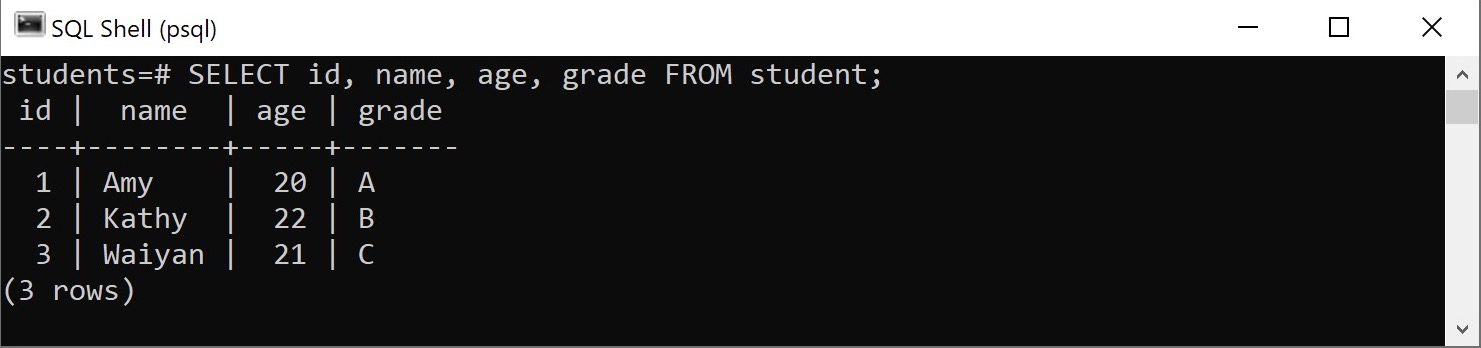
\includegraphics[width=.98\textwidth, trim={0mm 0.5mm 0.5mm 0.2mm}]{images/ch12/select.jpg}};
  \drawshadow{image}
\end{tikzpicture}
\caption{} 
\label{fig:selectstu}
\end{figure}

\fEn{Column} အကုန်မထုတ်ဘဲ ကိုယ်လိုချင်တာပဲ ရွေးပြီး \fEn{select} လုပ်ချင်လည်း ရတယ်။ အောက်ပါတို့ကို \fEn{psql} မှာ စမ်းကြည့်ပါ။
%
\begin{sql}
SELECT name, grade FROM student;
SELECT name, age, id FROM student;
\end{sql}
%
\subsection*{\fSubSecCodeBf{WHERE}}
\fEn{Grade A} ရတဲ့ ကျောင်းသားတွေကိုပဲ ရွေးထုတ်ကြည့်မယ် ဆိုပါစို့။ ဒီအတွက် \fEn{SQL} မှာ \fCode{WHERE} ရှိပါတယ်။ ဥပမာ
%
\begin{sql}
SELECT * FROM student WHERE grade = 'A';
\end{sql}
%
\fCode{WHERE} နောက်မှာ ဘူလီယန် အိပ်စ်ပရက်ရှင်တစ်ခု ပါရပါမယ်။ \fCode{WHERE} ကွန်ဒီရှင် \fEn{(Condition)} လို့ခေါ်တယ်။ ရေးပုံရေးနည်း နည်းနည်းကွာပေမဲ့ \fEn{SQL} \fCode{WHERE} ကွန်ဒီရှင် က \fEn{Python} ဘူလီယန် အိပ်စ်ပရက်ရှင်နဲ့ သဘောတရားအားဖြင့် တူပါတယ်။ \fCode{grade = 'A'} က \fCode{grade} \fEn{column} တန်ဖိုး \fCode{'A'} နဲ့ ညီလား စစ်တာ။ ညီတဲ့ \fEn{record} တွေကိုပဲ \fCode{WHERE} က စစ်ထုတ်ပေးမှာပါ။ ဒါ့ကြောင့် အပေါ်က \fCode{select} က \fEn{record} တစ်ကြောင်းပဲ ထွက်မှာပါ။ အေမီတစ်ယောက်ပဲ \fEn{A} ရပါတယ်။ \fCode{WHERE} နဲ့ပါတ်သက်ပြီး လက်တွေ့စမ်းကြည့်ရအောင် အောက်ပါအတိုင်း ကျောင်းသား \fEn{record} လေးခု ထပ်ထည့်ပါမယ်။  
%
\begin{sql}
INSERT INTO student (name, age, grade) VALUES ('Sandy', 19, 'A');
INSERT INTO student (name, age, grade) VALUES ('Thida', 21, 'B');
INSERT INTO student (name, age, grade) VALUES ('Peter', 21, 'B');
INSERT INTO student (name, age, grade) VALUES ('Haymar', 18, NULL);
\end{sql}
%

\fEn{Grade A} သို့ \fEn{B} ရတဲ့ ကျောင်းသား \fEn{record} တွေ \fEn{select} လုပ်ဖို့ \fCode{OR} သုံးထားတာပါ။ \fEn{psql} မှာ စမ်းကြည့်ပါ။ \fEn{Amy, Kathy, Sandy, Thida, Peter} တို့ \fEn{A} သို့ \fEn{B} ရကြတယ်။
%
\begin{sql}
SELECT * FROM student WHERE grade = 'A' OR grade = 'B';
\end{sql}
\fEn{Grade A} သို့ \fEn{B} မရတဲ့ ကျောင်းသားတွေ ထုတ်ချင်ရင် \fCode{NOT} နဲ့ အခုလို ရတယ်
%
\begin{sql}
SELECT name FROM student WHERE NOT(grade = 'A' OR grade = 'B');
\end{sql}
ဝေယံ တစ်ယောက်ပဲ ရလဒ်မှာတွေ့ရမှာပါ။ ဟေမာ ဘာကြောင့် မပါရတာလဲ။ စဉ်းစားကြည့်ရင် သူမ \fEn{A} လည်းမရ၊ \fEn{B}  လည်းမရဘူး။ ဒါကြောင့်  ပါသင့်တယ် ယူဆကောင်း ယူဆနိုင်တယ်။ \fCode{NULL} ဟာ မရှိခြင်း၊ မသိခြင်း ကိုဖော်ပြဖို့ \fEn{SQL} မှာ အသုံးပြုတဲ့ \fEn{special value} တစ်ခု ဖြစ်ပါတယ်။ ဟေမာ့ \fEn{grade} က \fCode{NULL} ဖြစ်နေတယ်။ ဆိုလိုတာက သူ့ \fEn{grade} ကို မသိဘူး။ 

\fCode{NULL} နဲ့ အခြားတန်ဖိုးတစ်ခုခု ညီ/မညီ စစ်တဲ့အခါ ရလဒ်က \fCode{NULL} ပဲ ဖြစ်ပါတယ်။ အဓိပ္ပါယ်က ညီ/မညီ ‘မသိဘူး’ ဆိုတဲ့ အဓိပ္ပါယ်။ ဒါ့ကြောင့် ဘူလီယန် အိပ်စ်ပရက်ရှင် \fCode{'A' = NULL} ရဲ့ အဖြေ \fCode{NULL} ဖြစ်သလို \fCode{'A' <> NULL} ရဲ့ အဖြေလည်း \fCode{NULL} ပဲ ဖြစ်တယ်။ 

\fEn{Select} လုပ်တဲ့အခါ \fCode{WHERE} ကွန်ဒီရှင် \fEn{true} ဖြစ်တဲ့ \fEn{record} တွေကို ရွေးထုတ်ပေးတယ်။ \fCode{WHERE} ကွန်ဒီရှင် ရလဒ်တန်ဖိုး \fCode{NULL} ဖြစ်ရင် အဲဒီ \fEn{record} ကို ထုတ်ပေးမှာ မဟုတ်ဘူး။ စောစောက \fEn{select} ရလဒ်မှာ ဟေမာ ဘာ့ကြောင့်  မပါလဲ အောက်ပါအတိုင်း စဉ်းစားကြည့်နိုင်ပါတယ်%
%
\begin{align*}
         &\text{\fEn{WHERE NOT(\textit{NULL} = \`{}A\`{} OR \textit{NULL} = \`{}B\`{})}}\\
\implies &\text{\fEn{WHERE NOT(\textit{NULL} OR \textit{NULL})}}\\
\implies &\text{\fEn{WHERE NOT(\textit{NULL})}}\\
\implies &\text{\fEn{WHERE \textit{NULL}}}\\
\end{align*}%

\fEn{Grade C} မဟုတ်တဲ့ ကျောင်းသားတွေကို အောက်ပါအတိုင်း နည်းလမ်းနှစ်မျိုးနဲ့ \fEn{select} လုပ်ကြည့်ပါ။ အခုတစ်ခါလည်း ဟေမာ ရလဒ်မှာ မပါတာကို သတိပြုပါ။
%
\begin{sql}
SELECT * FROM student WHERE grade <> 'C';
\end{sql}
%
%
\begin{sql}
SELECT * FROM student WHERE NOT(grade = 'C');
\end{sql}
%
ဒီတစ်ခု ထပ်စမ်းကြည့်ပါ။ ရှင်းပြဖို့မလိုဘဲ အဓိပ္ပါယ် နားလည်မယ် ထင်ပါတယ်။
%
\begin{sql}
SELECT * FROM student WHERE grade = 'B' AND id <= 5;
\end{sql}
%

\fCode{NULL} ဟုတ်/မဟုတ် စစ်ချင်ရင် \fEn{SQL} မှာ \fCode{IS NULL} (သို့) \fCode{IS NOT NULL}  သုံးရပါတယ်။ \fCode{=} နဲ့ \fCode{<>} ကို သုံးလို့မရဘူး။ မှားယွင်း အသုံးပြုမိတတ်လို့ ဒီအချက်ကို အထူးဂရုပြုရပါမယ်။ \fEn{Grade} \fCode{NULL} ဖြစ်တဲ့ \fEn{record} တွေနဲ့ \fCode{NULL} မဟုတ်တဲ့ \fEn{record} တွေကို အခုလို ရွေးထုတ်နိုင်ပါတယ်။
%
\begin{sql}
SELECT * FROM student WHERE grade IS NULL;
SELECT * FROM student WHERE grade IS NOT NULL;
\end{sql}
%
\fEn{Grade} \fCode{NULL} ဖြစ်တာ ဟေမာတစ်ယောက်ပဲ ရှိတာမို့လို့ ပထမ \fEn{select} က \fEn{record} တစ်ကြောင်းပဲ ထွက်မှာပါ။ အောက်ပါအတိုင်း တစ်ဆင့်ချင်း စဉ်းစားကြည့်ပါ
\begin{align*}
    &\text{\fEn{WHERE grade IS \textit{NULL}}}\\
\implies &\text{\fEn{WHERE \textit{NULL} IS \textit{NULL}}}\\
\implies &\text{\fEn{WHERE TRUE}}\\
\end{align*}
ဒုတိယ \fEn{select} မှာ ကျတော့ ဘာကြောင့် ဟေမာ မပါလဲ။ ကျန်တဲ့သူတွေကရော ဘာကြောင့်ပါလဲ။ အောက်ပါအတိုင်း တစ်ဆင့်ချင်း စဉ်းစားကြည့်ပါ။ ဟေမာ့ \fEn{record} အတွက်%
%
\begin{align*}
    &\text{\fEn{WHERE grade IS NOT \textit{NULL}}}\\
\implies &\text{\fEn{WHERE \textit{NULL} IS NOT \textit{NULL}}}\\
\implies &\text{\fEn{WHERE FALSE}}\\
\end{align*}
\fEn{A} ရထားတဲ့ ကျောင်းသား \fEn{record} ဆိုရင် ဒီလို 
\begin{align*}
    &\text{\fEn{WHERE grade IS NOT \textit{NULL}}}\\
\implies &\text{\fEn{WHERE \`{}A\`{} IS NOT \textit{NULL}}}\\
\implies &\text{\fEn{WHERE TRUE}}\\
\end{align*}
အခြား \fCode{NULL} မဟုတ်တဲ့ \fEn{grade} အားလုံးအတွက် အလားတူဖြစ်မယ်။ ဒါ့ကြောင့် ဒုတိယ \fEn{select} ရလဒ်မှာ ဟေမာကလွဲလို့ ကျန်တဲ့သူအားလုံး ပါလာတာဖြစ်တယ်။

\subsection*{\fSubSecCodeBf{ORDER BY}}
\fCode{ORDER BY} က \fEn{record} တွေကို \fEn{column} တန်ဖိုးပေါ် မူတည်ပြီး ‘အစဉ်အတိုင်းစီခြင်း’ \fEn{(sorting)} အတွက်ပါ။
%
\begin{sql}
SELECT * FROM student ORDER BY grade;
\end{sql}
%
\fEn{Grade} အလိုက် \fEn{order by} လုပ်ထားတာပါ။ ရလဒ်ကို ပုံ (\fRefNo{\ref{fig:orderbyasc}}) မှာ ကြည့်ပါ။ ကြီးစဉ်ငယ်လိုက် စီချင်ရင် \fCode{DESC} \fEn{(descending)} နဲ့ ရတယ်။
\begin{figure}[tbh!]
\begin{tikzpicture}
  \node[anchor=south west,inner sep=0] (image) at (0,0)
  {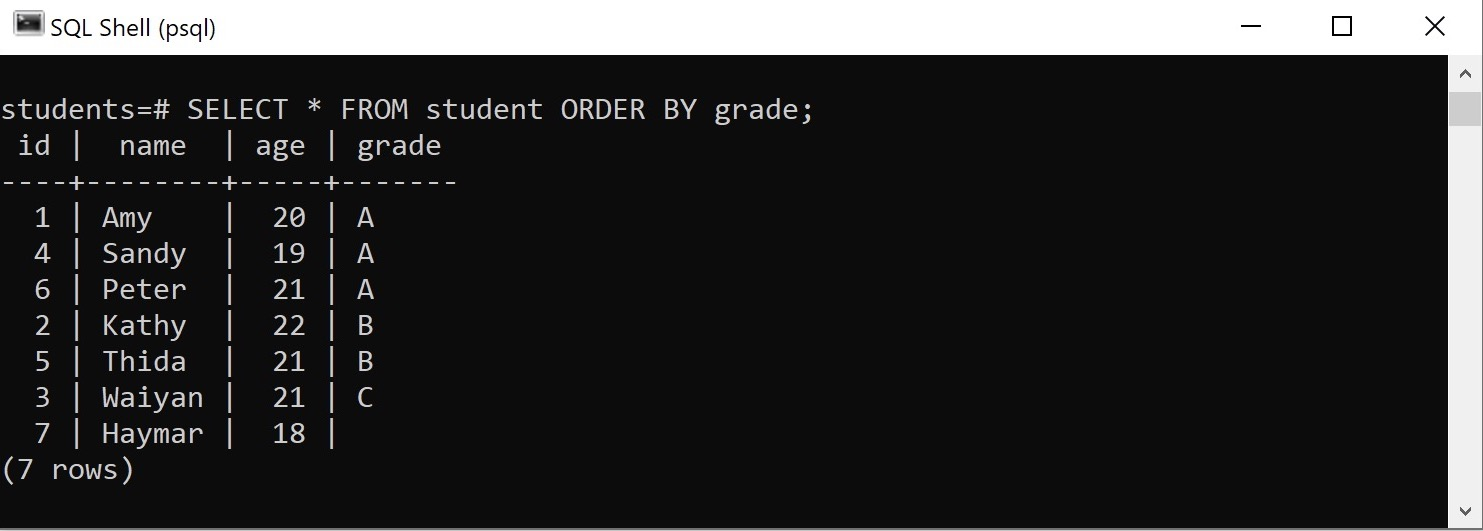
\includegraphics[width=.98\textwidth, trim={0mm 0.5mm 0.5mm 0.5mm},clip]{images/ch12/orderbyasc.jpg}};
  \drawshadow{image}
\end{tikzpicture}
\caption{} 
\label{fig:orderbyasc}
\end{figure}
%
\begin{sql}
SELECT * FROM student ORDER BY grade DESC;
\end{sql}
%
သူ့ နဂို \fEn{default} ကတော့ \fCode{ASC} \fEn{(ascending)} ပါ။ 

\fEn{Column} တစ်ခုမကနဲ့  စီချင်လည်း ရတယ်။ \fCode{ORDER BY} နောက်မှာ \fEn{sort} လုပ်ရမဲ့ \fEn{column} တွေ ထည့်ပေးရုံပဲ။ \fEn{Age} နဲ့ \fEn{grade} တွဲရက် \fEn{sort} လုပ်မယ်ဆိုရင်
%
\begin{sql}
SELECT * FROM student ORDER BY age, grade;
\end{sql}
%
\fEn{psql} ရလဒ်မှာ အောက်ပါအတိုင်း တွေ့ရမှာပါ။ \fEn{Thida, Peter, Waiyan} တို့ကို သေချာ ဂရုပြုကြည့်ပါ။ \fEn{Age} တူရင် \fEn{grade B} ရတဲ့သူက အရင်လာတာကို တွေ့ရပါမယ်။ \fEn{Grade C} က နောက်မှာပါ။
\begin{vbtm}
ß\fEnBf{Output:}ß
 id |  name  | age | grade
----+--------+-----+-------
  7 | Haymar |  18 |
  4 | Sandy  |  19 | A
  1 | Amy    |  20 | A
  5 | Thida  |  21 | B
  6 | Peter  |  21 | B
  3 | Waiyan |  21 | C
  2 | Kathy  |  22 | B
(7 rows)
\end{vbtm}
\fEn{Name} ထပ်ထည့်ကြည့်ပါ။  \fEn{Peter} က \fEn{Thida} ရဲ့ ရှေ့ရောက်သွားတာကလွဲလို့ ခုနက စီထားတာနဲ့ အားလုံးတူပါမယ်။
%
\begin{sql}
SELECT * FROM student ORDER BY age, grade, name;
\end{sql}
%

\fEn{Age} နဲ့ \fEn{grade} ကို ရှေ့‌နောက် ပြောင်းကြည့်ပါ။ 
%
\begin{sql}
SELECT * FROM student ORDER BY grade, age;
\end{sql}
%
\fEn{Grade} \fEn{A, B, C} အစဉ်အတိုင်း ဖြစ်မယ်။ \fEn{Grade} တူရင်တော့ \fEn{age} ငယ်တဲ့ \fEn{record} က ရှေ့ရောက်ပါတယ်။ အခုလို စီသွားမှာပါ
%
\begin{vbtm}
ß\fEnBf{Output:}ß
 id |  name  | age | grade
----+--------+-----+-------
  4 | Sandy  |  19 | A
  1 | Amy    |  20 | A
  5 | Thida  |  21 | B
  6 | Peter  |  21 | B
  2 | Kathy  |  22 | B
  3 | Waiyan |  21 | C
  7 | Haymar |  18 |
(7 rows)
\end{vbtm}
%

\fEn{Grade} ကို \fCode{DESC} နဲ့ \fEn{age} ကို \fCode{ASC} ထားကြည့်ပါ။ ခုနကဟာနဲ့ ဘာကွာခြားလဲ သေချာဂရုပြု လေ့လာကြည့်ပါ။
%
\begin{sql}
SELECT * FROM student ORDER BY grade DESC, age ASC;
\end{sql}
%
\begin{vbtm}
ß\fEnBf{Output:}ß
 id |  name  | age | grade
----+--------+-----+-------
  7 | Haymar |  18 |
  3 | Waiyan |  21 | C
  6 | Peter  |  21 | B
  5 | Thida  |  21 | B
  2 | Kathy  |  22 | B
  4 | Sandy  |  19 | A
  1 | Amy    |  20 | A
(7 rows)
\end{vbtm}

\fCode{ORDER BY} နဲ့ စီတဲ့အခါ \fCode{ORDER BY} နောက်မှာ \fEn{list} လုပ်ထားတဲ့ \fEn{column} အစီအစဉ်နဲ့ \fCode{ASC}\fEn{,} \fCode{DESC} တို့ကို လိုသလို အသုံးပြုပြီး လိုချင်တဲ့အတိုင်း ရအောင် \fEn{sort} လုပ်လို့ရပါတယ်။ ပရိုဂရမ်းမင်းမှာရော ဒေတာဘေ့စ်ပိုင်းမှာပါ \fEn{sorting} စီခြင်းဟာ အရေးကြီးတာကြောင့် ကျွမ်းကျင်အောင် လုပ်ထားသင့်ပါတယ်။


\subsection*{\fSubSecCodeBf{UPDATE}}
\fEn{Table record} တွေ \fEn{update} လုပ်ဖို့ အသုံးပြုတဲ့ \fEn{SQL} စတိတ်မန့် ဖြစ်ပါတယ်။ \fCode{id} နံပါတ် \fEn{7} နဲ့ \fEn{record} ရဲ့ \fEn{grade} နဲ့ \fEn{age} ကို \fEn{update} လုပ်တဲ့ ဥပမာ
%
\begin{sql}
UPDATE student SET grade = 'A', age = 19 WHERE id = 7;
\end{sql}
%
\fCode{WHERE} ပါရင် \fCode{WHERE} ကွန်ဒီရှင်နဲ့ ကိုက်ညီတဲ့ \fEn{record} ကိုပဲ \fEn{update} လုပ်တယ်။ အခု \fEn{update} စတိတ်မန့်က \fCode{id} \fEn{7} နဲ့ က ဟေမာ့ \fEn{record} တစ်ခုကိုပဲ \fEn{update} လုပ်မှာပါ။ အကယ်၍ \fCode{WHERE} မပါခဲ့ရင် \fEn{table} မှာရှိတဲ့ \fEn{record} တွေ အကုန်လုံးကို \fEn{update} လုပ် သွားလိမ့်မယ်။

%
\begin{sql}
UPDATE student SET grade = 'A+' WHERE id IN (1, 4, 6);
\end{sql}
%
\fCode{id} နံပါတ်က $(1,4,6)$ ထဲမှာပါရင် \fEn{grade} ကို \fEn{A+} \fEn{update} လုပ်ထားတာပါ။ \fCode{WHERE} ကွန်ဒီရှင်မှာ \fCode{IN}  အော်ပရိတ်တာ သုံးထားတယ်။ \fEn{Column} တစ်ခုရဲ့ တန်ဖိုးဟာ \fEn{list} လုပ်ထားတဲ့ တန်ဖိုးတွေထဲမှာ ပါ/မပါ စစ်ချင်ရင် \fCode{IN} သုံးပါတယ်။ \fEn{Update} လုပ်ထားတဲ့ \fEn{record} တွေကို \fEn{select} လုပ်ကြည့်ပါ။ 
%
\begin{sql}
SELECT * FROM student WHERE id IN (1, 4, 6, 7);
\end{sql}
%
ပုံ (\fRefNo{\ref{fig:afterupdate}}) မှာလို တွေ့ရပါမယ်။

\begin{figure}[tbh!]
\begin{tikzpicture}
  \node[anchor=south west,inner sep=0] (image) at (0,0)
  {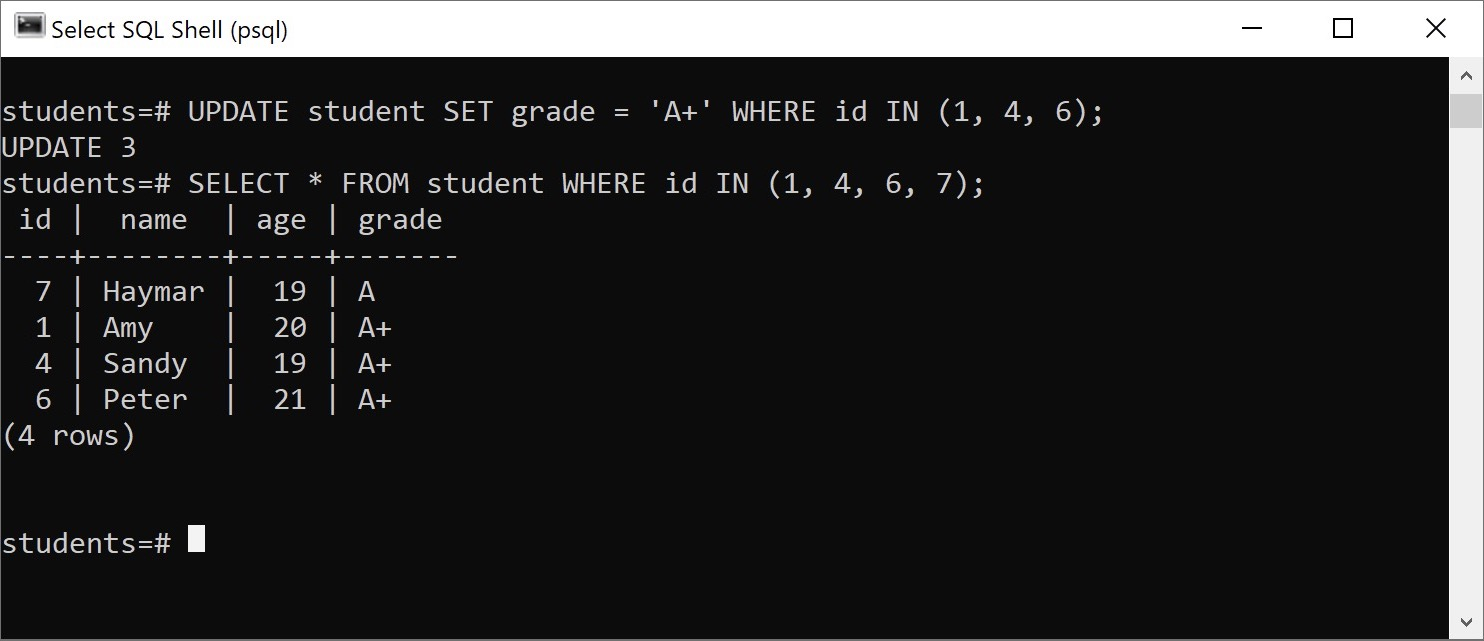
\includegraphics[width=.98\textwidth, trim={0mm 50mm 0.5mm 0.5mm},clip]{images/ch12/afterupdate.jpg}};
  \drawshadow{image}
\end{tikzpicture}
\caption{} 
\label{fig:afterupdate}
\end{figure}

\subsection*{\fSubSecCodeBf{DELETE}}
\fEn{Table row} တွေ ဖျက်ဖို့ အသုံးပြုတဲ့ စတိတ်မန့် ဖြစ်ပါတယ်။ \fEn{Student table} ထဲက \fEn{record} အားလုံး ဖျက်မယ်ဆိုရင် အခုလို ဖျက်ရမှာပါ
%
\begin{sql}
DELETE FROM students;
\end{sql}
%
\fEn{Development/testing} ဒေတာဘေ့စ်မှာ \fEn{table} ဒေတာ အကုန်ဖျက်ပြီး အစမ်းဒေတာ \fEn{(test data)} ပြန်ထည့်ဖို့ ဒီလို လုပ်ရလေ့ရှိပေမဲ့ တကယ်သုံးနေတဲ့ \fEn{production} ဒေတာဘေ့စ်မှာတော့ \fEn{table} ဒေတာ အကုန်ဖျက်ပစ်ရမဲ့ အခြေအနေဆိုတာ ကြုံတောင့်ကြုံခဲပါပဲ။ \fCode{WHERE} နဲ့ ဖျက်ရမဲ့ \fEn{record} ကို ရွေးပြီး ဖျက်တာက ပိုပြီး သဘာဝကျပါတယ်။ ဝေယံ ကျောင်းထွက်သွားလို့ သူ့ \fEn{record} ကို သိမ်းထားဖို့ မလိုတော့ဘူး ဆိုပါစို့၊ အခုလို 
%
\begin{sql}
DELETE FROM student WHERE id = 3;
\end{sql}
%
\fEn{delete} လုပ်နိုင်ပါတယ် (\fEn{id} နံပါတ် \fEn{3} နဲ့ \fEn{record} က ဝေယံ)။

\section{Table Relationships}
ဒေတာဘေ့စ် တစ်ခုမှာ \fEn{table} တစ်ခုမက \fEn{(multiple tables)} ပါဝင် ဖွဲ့စည်းထားလေ့ ရှိတယ်။ \fEn{Table} တွေနဲ့ ၎င်းတို့ကြား \fEnEmp{relationship} ဟာ \fEn{Relational Data Model} ရဲ့ အဓိကကျတဲ့ သဘောတရားဖြစ်တယ်။ သက်ဆိုင်\allowbreak ရာ \fEn{table} အသီးသီးမှာ အချက်အလက်တွေ စုစည်းသိမ်းဆည်းပုံ သိမ်းဆည်းနည်း စနစ်ကို လေ့လာကြရအောင်။ 

ဘဏ်တစ်ခုကို စိတ်ကူးကြည့်ပါ။ ဘဏ်အကောင့်၊ အကောင့်ပိုင်ရှင်နဲ့ ငွေဝင်ငွေထွက် စာရင်း အချက်\allowbreak အလက်တွေ သိမ်းဆည်းမယ် ဆိုပါစို့။ \fEn{Table} တစ်ခုတည်းနဲ့ အားလုံးသိမ်းလို့ ရပေမဲ့ \fEn{Relational Data Model} အရ \fEn{table} သုံးခုခွဲပြီး သီးခြားစီသိမ်းတာ ပိုကောင်းပါတယ်။  အကောင့်ပိုင်ရှင်နဲ့ သက်ဆိုင်တဲ့ အချက်အလက်တွေအတွက် \fEn{table} တစ်ခု ရှိပါမယ်။
%
\begin{sql}
CREATE TABLE account_holder (
    holder_id SERIAL PRIMARY KEY,
    fname VARCHAR(50),
    lname VARCHAR(50),
    dob DATE,
    address TEXT
);
\end{sql}
%
အကောင့်နဲ့ သက်ဆိုင်တဲ့ အချက်အလက်တွေအတွက် သီးခြား \fEn{table} တစ်ခုရှိမယ်။ (လောလောဆယ် ဒီ \fEn{table} နှစ်ခုကို အရင်ကြည့်ရအောင်၊ ငွေဝင်ငွေထွက် စာရင်းနဲ့ ဆိုင်တဲ့ တတိယ \fEn{table} ကို နောက်ပိုင်းမှာ တွေ့ရမှာပါ)။ 
%
\begin{sql}
CREATE TABLE account (
    acc_id SERIAL PRIMARY KEY,
    holder_id INT REFERENCES account_holder(holder_id),
    acc_no VARCHAR(20) UNIQUE,
    acc_type VARCHAR(20),
    balance NUMERIC(12, 2) DEFAULT 0.00
);
\end{sql}
%
ဒီ \fCode{account} \fEn{table} မှာ \fCode{holder\_id} \fEn{column} က \fCode{account\_holder} \fEn{table} ရဲ့ \fCode{holder\_id} \fEn{column} ကို ရည်ညွှန်းထားပါတယ်။ အကောင့်နဲ့ အကောင့် ပိုင်ရှင် အချက်အလက်တွေကို ဒီ \fEn{table} နှစ်ခုမှာ ဘယ်လို ဆက်စပ် သိမ်းဆည်းလဲ နားလည်အောင် နမူနာ \fEn{record} အနည်းငယ်ထည့်ပြီး ရှင်းပြပါမယ်။ အောက်ပါအတိုင်း \fEn{insert} လုပ်ပါ။
%
\begin{sql}
INSERT INTO account_holder (fname, lname, dob, address)
VALUES 
('Amy', 'Moe', '1985-02-15', '123 Main St, Sanchaung'),
('Sandy', 'Soe', '1990-06-23', '456 Oak St, Kamayaut');
\end{sql}
%
\fEn{Insert} လုပ်ပြီးရင် အေမီနဲ့ စန္ဒီ့ \fCode{holder\_id} နံပါတ်က $1$ နဲ့ $2$ အသီးသီး ဖြစ်မယ်။ အေမီဖွင့်ထားတဲ့ အကောင့်နှစ်ခုနဲ့ စန္ဒီရဲ့ အကောင့်တစ်ခုကို အောက်ပါအတိုင်း \fCode{account} \fEn{table} မှာ သိမ်းနိုင်ပါတယ်။ \fCode{holder\_id} $1$ နဲ့ $2$ ကို အထူး ဂရုပြုပါ။
%
\begin{sql}
INSERT INTO account (holder_id, acc_no, acc_type, balance)
VALUES 
(1, '0086-6002-1111', 'Savings', 500000.00),
(1, '0088-6005-1122', 'Current', 800000.00),
(2, '0086-6002-3311', 'Savings', 400000.00);
\end{sql}
%
ဒီ \fEn{table} မှာ ကြည့်ရင် အကောင့်ပိုင်ရှင် အသေးစိတ်အချက်အလက်ကို မတွေ့ရပါဘူး။ အကောင့် \fEn{record} တစ်ခုစီအတွက်  ပိုင်ရှင်ရဲ့ \fCode{holder\_id} ကိုပဲ တွေ့ရမှာပါ။ ဒီ \fCode{holder\_id} ဟာ \fCode{account\_holder} \fEn{table} ထဲက \fEn{record} တစ်ခုရဲ့ \fCode{holder\_id} ကို ရည်ညွှန်းရပါမယ်။ 

ပထမ အကောင့်နှစ်ခု \fCode{holder\_id} က $1$ ဖြစ်တယ်။ \fCode{account\_holder} \fEn{table} မှာပြန်ကြည့်ရင် \fCode{holder\_id} $1$ က အေမီ။ ဒါကြောင့် ဒီအကောင့်နှစ်ခုဟာ အေမီ့ရဲ့ အကောင့်ဖြစ်တယ်။ ထိုနည်းတူစွာ \fCode{holder\_id} $2$ က စန္ဒီဖြစ်တဲ့အတွက် တတိယအကောင့်ဟာ သူမရဲ့ အကောင့်ဖြစ်တယ်လို့ သိနိုင်ပါတယ်။ အခု ဖော်ပြခဲ့သလို အချက်အလက် သိမ်းဆည်းပုံ နည်းစနစ်ဟာ \fEn{Relational Model} ရဲ့ အဓိကကျတဲ့ အခြေခံ သဘောတရားလို့ ဆိုရမှာပါ။

\subsection*{Table \fSubSecCodeBf{JOIN}}
\fEn{Table} နှစ်ခုကို ပေါင်းစပ်ကြည့်ရင် အကောင့်ရော အကောင့်ပိုင်ရှင် အချက်အလက်ကိုပါ အပြည့်အစုံ သိနိုင်မှာပါ။ ဥပမာ အခုလို \fEn{select} လုပ်ကြည့်ရင် အေမီနဲ့ သူမ၏အကောင့် အသေးစိတ် အချက်အလက်တွေကို တွေ့ရပါမယ်
%
\begin{sql}
SELECT * FROM account_holder WHERE holder_id = 1;
SELECT * FROM account WHERE holder_id = 1;
\end{sql}
%
\begin{vbtm}
ß\fEnBf{Output:}ß
 holder_id | fname | lname |    dob     |        address
-----------+-------+-------+------------+------------------------
         1 | Amy   | Moe   | 1985-02-15 | 123 Main St, Sanchaung
(1 row)


 acc_id | holder_id |     acc_no     | acc_type |  balance
--------+-----------+----------------+----------+-----------
      1 |         1 | 0086-6002-1111 | Savings  | 500000.00
      2 |         1 | 0088-6005-1122 | Current  | 800000.00
(2 rows)
\end{vbtm}

\fEn{Table} နှစ်ခု ချိတ်ဆက်ပြီး အကောင့်နဲ့ အကောင့်ပိုင်ရှင် တစ်ဆက်တည်း ထုတ်ကြည့်မယ် ဆိုရင်တော့ ဒီအတွက် \fEn{SQL} \fCode{JOIN} ရှိပါတယ်။
%
\begin{sql}
SELECT * FROM account_holder JOIN account
ON account_holder.holder_id = account.holder_id;
\end{sql}
%
\fEn{Psql} မှာ စမ်းကြည့်ရင် အခုလို ရမှာပါ

\begin{figure}[H]
\begin{tikzpicture}
  \node[anchor=south west,inner sep=0] (image) at (0,0)
  {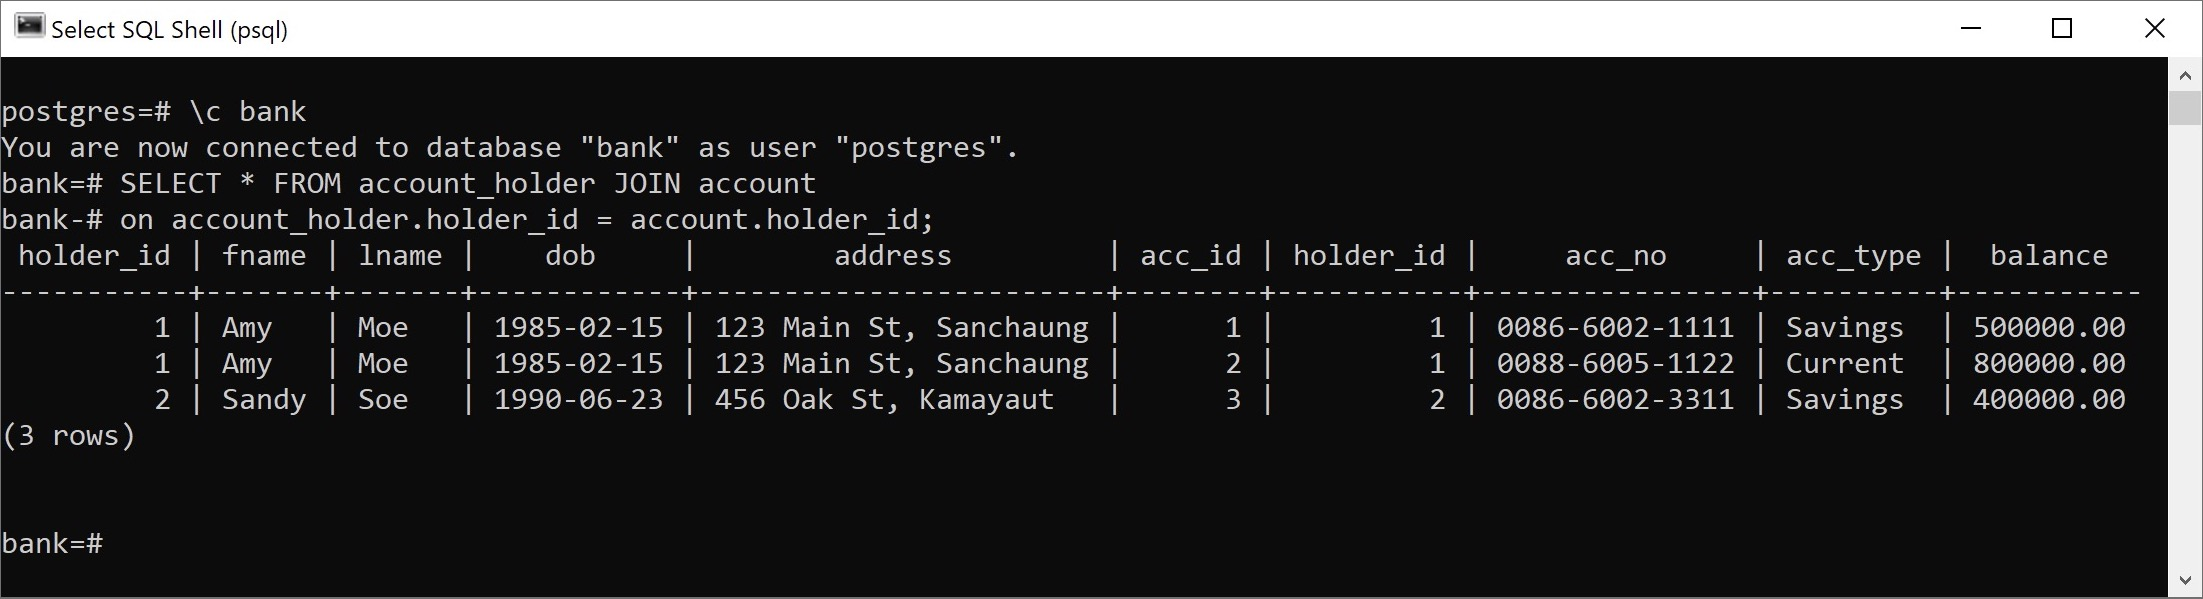
\includegraphics[width=1.13\textwidth, trim={0mm 50mm 0mm 0.5mm},clip]{images/ch12/join.jpg}};
  \drawshadow{image}
\end{tikzpicture}
\caption{} 
\label{fig:join}
\end{figure}
\fCode{account\_holder} \fEn{table} ရဲ့ \fCode{holder\_id} နဲ့  \fCode{account} \fEn{table} ရဲ့ \fCode{holder\_id} တူရင် \fCode{JOIN} က \fEn{record} တွေကို တွဲဆက်ပေးတာ တွေ့ရမှာပါ။ တွဲဆက်ပေးရမဲ့ ကွန်ဒီရှင်ကို \fCode{ON} နောက်မှာ အခုလို ထည့်ပေးထားတယ်
%
\begin{sql}
ON account_holder.holder_id = account.holder_id;
\end{sql}
%
\fCode{JOIN} ကို နောက်ပုံစံတစ်မျိုးနဲ့ ရေးလို့လည်း ရတယ်။ \fCode{account\_holder} \fEn{table} ကို \fCode{t1} နဲ့၊ \fCode{account} ကို \fCode{t2} နဲ့ ရည်ညွှန်းပါတယ်။ \fEn{Alias} လုပ်တာလို့ ခေါ်ပါတယ်။
%
\begin{sql}
SELECT 
    t1.*,
    t2.* 
FROM account_holder t1 JOIN account t2
    ON t1.holder_id = t2.holder_id;
\end{sql}
%
\fEn{Table} နှစ်ခုကနေ လိုချင်တဲ့ \fEn{column} ကိုပဲ ရွေးထုတ်လည်း ရတယ်။ ဥပမာ
%
\begin{sql}
SELECT 
    t2.*,
    t1.fname,
    t1.lname
FROM account_holder t1 JOIN account t2
    ON t1.holder_id = t2.holder_id;
\end{sql}
%

\subsection*{Referential Integrity}
\fEn{Relational Model} ဟာ \fEnEmp{referential integrity} ကို မပျက်ယွင်းအောင် အလေးအနက်ထား  ထိန်းသိမ်းပေးပါတယ်။ \fEn{Record} တစ်ခုကို ဖျက်တဲ့အခါ အဲဒီဖျက်လိုက်တဲ့ \fEn{record} ကို အခြား \fEn{table} မှာရှိတဲ့ \fEn{record} တွေက ရည်ညွှန်းထားမယ်ဆိုရင် ပြဿနာရှိတယ်။ ဥပမာ \fCode{account\_holder} \fEn{table} မှာ အကောင့်ပိုင်ရှင် အေမီ့ \fEn{record} ကို ဖျက်လိုက်တယ် ဆိုပါစို့။ ဒီလိုဆိုရင် \fCode{account} \fEn{table} ထဲက \fCode{holer\_id} $1$ နဲ့ အကောင့်နှစ်ခု ရည်ညွှန်းထားတဲ့ အကောင့်ပိုင်ရှင် \fEn{record} ရှိမှာ မဟုတ်တော့ဘူး။ ဒါဟာ \fEn{referential integrity} ကို ချိုးဖောက်တာ ဖြစ်တဲ့အတွက် \fEn{Relational Model} က အဲဒီလို ဖျက်ခွင့်ပေးမှာ မဟုတ်ပါဘူး။ \fEn{Record} တစ်ခုကို အခြား \fEn{record} တွေက \fEn{reference} လုပ်ထားတာ ရှိနေသ၍ \fEn{Relational Model} က အဲ့ဒီ \fEn{record} ပေးမဖျက်ဘူး။ အခုလို စမ်းပြီး ဖျက်ကြည့်ပါ။ 
%
\begin{figure}[tbh!]
\begin{tikzpicture}
  \node[anchor=south west,inner sep=0] (image) at (0,0)
  {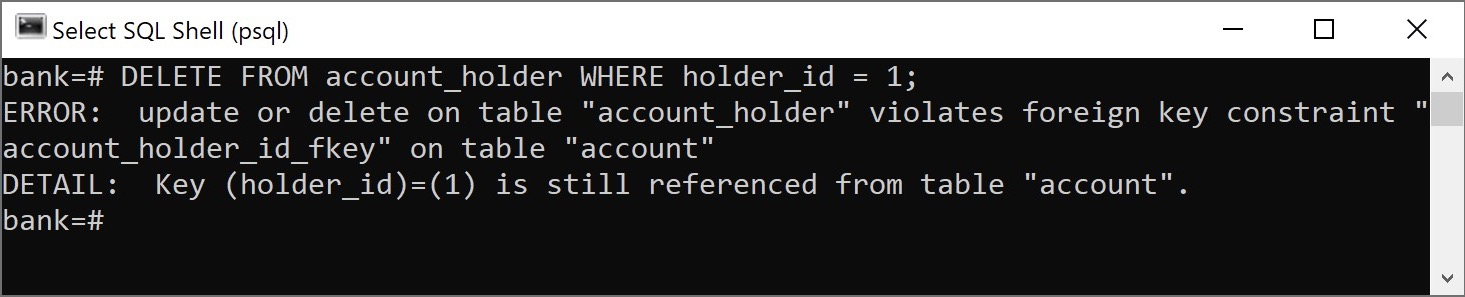
\includegraphics[width=.98\textwidth, trim={0.5mm 0mm 0mm 0.8mm},clip]{images/ch12/ref_integrity.jpg}};
  \drawshadow{image}
\end{tikzpicture}
\caption{} 
\label{fig:ref_integrity}
\end{figure}%
ဖျက်ခွင့်မပေးတာကို တွေ့ရပါလိမ့်မယ်။

\fCode{holer\_id} $1$ နဲ့ \fEn{record} ကို ဖျက်ချင်ရင် ၎င်းကို ရည်ညွှန်းတဲ့ \fEn{record} တွေကို အရင်ဖျက်ရပါမယ်။ ဒါမှမဟုတ် နောက်ထပ်နည်းလမ်းတစ်ခုက \fEn{parent record} ကိုဖျက်ရင် ဆက်စပ်နဲ့တဲ့ \fEn{child record} တွေကိုပါ အလိုအလျောက် ဖျက်အောင် \fCode{ON DELETE CASCADE} \fEn{option} အသုံးပြုတာပါ။ ရည်ညွှန်းတဲ့ \fEn{table/record} ကို \fEn{child table/record} လို့ ယူဆပါ။ ရည်ညွှန်းခြင်း ခံရတဲ့ \fEn{table/record} ကို \fEn{parent table/record} လို့ ယူဆပါ။ \fCode{ON DELETE CASCADE} ကို \fEn{child table} ဆောက်တဲ့အခါ \fCode{holder\_id} \fEn{column} မှာ အခုလို သတ်မှတ်ပေးရမှာပါ။
%
\begin{sql}
CREATE TABLE account (
    acc_id SERIAL PRIMARY KEY,
    holder_id INT REFERENCES account_holder(holder_id) ON DELETE CASCADE,
    ß$\ldots$ß
);
\end{sql}
%

\fEn{Referential integrity} နဲ့ ပါတ်သက်ပြီး နားလည်ထားဖို့ လိုပါတယ်။ ဒါကြောင့် အကျဉ်းချုံး ရှင်းပြထားတာပါ။ \fCode{ON DELETE CASCADE} စမ်းကြည့်မယ်ဆို ဒေတာဘေ့စ် ကိုဖျက်ပြီး \fEn{table} ပြန်ဆောက် (သို့) ဒေတာဘေ့စ် အသစ်တစ်ခု ဆောက်ပြီး စမ်းကြည့်ပါ။ ရှိပြီးသား \fEn{table} ကို \fCode{ON DELETE CASCADE} ဖြစ်အောင် လုပ်လို့ရပေမဲ့ နည်းနည်းပိုရှုပ်ထွေးပါတယ်။

\subsection*{Relationship Between \fSubSecCodeBf{account} and \fSubSecCodeBf{account\_transaction} Tables}
\fEn{Table relationship} နဲ့ \fCode{JOIN} ကို ပိုပြီး သဘောပေါက်အောင် အားဖြည့်တဲ့အနေနဲ့ နောက်ထပ် ဥပမာတစ်ခု ကြည့်ရအောင်။ အကောင့် ငွေသွင်း/ထုတ်စာရင်း \fEn{(account transaction)} \fEn{table} ပါ။
%
\begin{sql}
CREATE TABLE account_transaction (
    txn_id SERIAL PRIMARY KEY,
    -- reference to account table by acc_id
    acc_id INT REFERENCES account(acc_id),
    txn_date TIMESTAMP DEFAULT CURRENT_TIMESTAMP,
    txn_type VARCHAR(20),
    amount NUMERIC(12, 2),
    balance_after NUMERIC(12, 2)
);
\end{sql}
%
ဒီ \fEn{table} မှာ \fCode{acc\_id} \fEn{column} က \fCode{account} \fEn{table} ရဲ့ \fCode{acc\_id} \fEn{column} ကို \fEn{reference} လုပ်ထားတာကို ဂရုပြုကြည့်ပါ။ ငွေသွင်း/ထုတ် စာရင်း \fEn{(transaction)} ငါးခု အောက်ပါအတိုင်း ထည့်ပါမယ်။ 
%
\begin{sql}
INSERT INTO account_transaction 
    (acc_id, txn_date, txn_type, amount, balance_after)
VALUES 
    (1, '2024-08-01 09:00:00', 'Deposit', 100000.00, 600000.00),
    (1, '2024-08-05 14:30:00', 'Withdrawal', 50000.00, 550000.00),
    (2, '2024-08-02 10:00:00', 'Deposit', 200000.00, 1000000.00),
    (2, '2024-08-03 16:00:00', 'Withdrawal', 300000.00, 700000.00),
    (3, '2024-08-04 11:00:00', 'Deposit', 50000.00, 450000.00);
\end{sql}
%
\fEn{Table} နှစ်ခုကို \fCode{acc\_id} နဲ့ ဘယ်လို ချိတ်ဆက်ထားလဲ နားလည်ဖို့ အရေးကြီးတယ်။ ပထမ \fEn{transaction} နှစ်ခုနဲ့ သက်ဆိုင်တဲ့ အကောင့် အချက်အလက် အသေးစိတ်ကို သိချင်ရင် \fCode{account} \fEn{table} မှာ \fCode{acc\_id} နံပါတ် $1$ နဲ့ \fEn{record} ကို ကြည့်ရမှာပါ
%
\begin{sql}
SELECT * FROM account WHERE acc_id = 1;
\end{sql}
%
%
\begin{vbtm}
ß\fEnBf{Output:}ß
 acc_id | holder_id |     acc_no     | acc_type |  balance
--------+-----------+----------------+----------+-----------
      1 |         1 | 0086-6002-1111 | Savings  | 500000.00
\end{vbtm}
%
\fCode{account\_transaction} \fEn{table} မှာ \fEn{transaction record} တွေ  \fEn{insert} လုပ်တဲ့အခါမှာလည်း ၎င်းတို့နှင့် သက်ဆိုင်တဲ့ \fCode{acc\_id} ကို မှန်ကန်အောင် သေချာစိစစ်ဖို့ လိုတယ်။ \fEn{Table} နှစ်ခုက အချက်အလက်တွေကို \fCode{JOIN} နဲ့ ချိတ်ဆက် ထုတ်ယူနိုင်တယ်။

%
\begin{sql}
SELECT 
    *
FROM account t1 JOIN account_transaction t2
    ON t1.acc_id = t2.acc_id;
\end{sql}
%
\fEn{Table} နှစ်ခုမကလည်း \fCode{JOIN} လို့ရတယ်။ ဥပမာ 
%
\begin{sql}
SELECT 
    t1.holder_id,
    t1.fname,
    t1.lname,
    t2.acc_no,
    t2.acc_type,
    t3.txn_type,
    t3.amount,
    t3.balance_after
FROM account_holder t1 JOIN account t2
    ON t1.holder_id = t2.holder_id
JOIN account_transaction t3
    ON t2.acc_id = t3.acc_id;
\end{sql}
%

\fEn{Table} သုံးခုကြား \fEn{relationship} ကို နားလည်အောင် နောက်ဆုံးတစ်ခါ အောက်ပါတို့ကို ဆက်စပ်ကြည့်ပါ။ \fEn{Insert} တစ်ခါလုပ်ပြီး \fEn{auto-generated id} နံပါတ်တွေ \fEn{select} လုပ်ကြည့်ပါ။
%
\begin{sql}
INSERT INTO account_holder (fname, lname, dob, address)
VALUES 
('Waiyan', 'Phyo', '1991-07-22', '45 Bawga St, Yankin');
\end{sql}
%
%
\begin{sql}
-- Before insert, make sure Waiyan's holder_id is 3
INSERT INTO account (holder_id, acc_no, acc_type, balance)
VALUES 
(3, '0086-6002-4411', 'Savings', 700000.00);
\end{sql}
%

%
\begin{sql}
-- Before insert, make sure Waiyan's acc_id is 4
INSERT INTO account_transaction 
    (acc_id, txn_date, txn_type, amount, balance_after)
VALUES 
    (4, '2024-08-05 15:45:00', 'Deposit', 200000.00, 900000.00);
\end{sql}
%


\section{SQL ဖန်ရှင်များ}
\fEn{SQL} မှာ \fEn{built-in} ဖန်ရှင်တွေ ပါရှိပါတယ်။ \fCode{to\_char}\fEn{,} \fCode{upper} နဲ့ \fCode{concat} သုံးထားတာ ကြည့်ပါ။ \fEn{Column} ကို \fEn{alias} ပေးလို့ရတယ်။ \fCode{Date\_of\_Birth} နဲ့ \fCode{Full\_Name} က \fEn{alias} တွေ။
%
\begin{sql}
SELECT
    to_char(dob, 'Mon DD YYYY') Date_of_Birth,
    upper(concat(fname, ' ', lname)) Full_Name
FROM account_holder;
\end{sql}
%
%
\begin{vbtm}
ß\fEnBf{Output:}ß
 date_of_birth |  full_name
---------------+-------------
 Feb 15 1985   | AMY MOE
 Jun 23 1990   | SANDY SOE
 Jul 22 1991   | WAIYAN PHYO
(3 rows)
\end{vbtm}
%
\fEn{SQL} \fCode{date} (သို့) \fCode{datetime} \fEn{data type} ကနေ လိုချင်တဲ့ \fEn{date/datetime format} ကို \fCode{to\_char} နဲ့ ပြောင်းလို့ရတယ်။ \fCode{'Mon DD YYYY'} က ဘယ်လို \fEn{format} လဲ သတ်မှတ်တာ။







\section{Database API}

\subsection*{\fSubSecCodeBf{psycopg2}}
% Psycopg is the most popular PostgreSQL database adapter for the Python programming language. 
\fEn{Python programming language} အတွက် \fEn{Psycopg} ဟာ \fEn{popular} အဖြစ်ဆုံး  \fEn{PostgreSQL} ဒေတာဘေ့စ် \fEn{adapter} ဖြစ်ပါတယ်။ ဒေတာဘေ့စ် \fEn{adapter} ဆိုတာ \fEn{DBMS} နဲ့ \fEn{programming language} ကြား ပေါင်းကူးတံတားအဖြစ် ဆောင်ရွက်ပေးတဲ့ လိုက်ဘရီပဲ ဖြစ်တယ်။

\fEn{Adapter} သုံးတဲ့အခါ \fEn{DBMS} နဲ့ \fEn{programming language} အလိုက် သက်ဆိုင်ရာ \fEn{adapter} ကို ရွေးချယ်ရမှာပါ။ \fEn{PostgreSQL} အတွက် \fEn{Python} မှာ \fEn{Psycopg 2} နဲ့ \fEn{Psycopg 3} ရှိမယ်။ အခြားဟာတွေလည်း ရှိပါသေးတယ်။ \fEn{MySQL} အတွက် \fEn{MySQL Connector/Python} သုံးကြတယ်။ \fEn{Microsoft SQL} အတွက်ဆိုရင် \fEn{pyodbc}။  

\subsection*{Connecting to PostgreSQL}
\fEn{Python} ကနေတစ်ဆင့် ဒေတာဘေ့စ် အသစ်တစ်ခု ဘယ်လိုဆောက်မလဲ ကြည့်ရအောင်။ စောစောက ပြောတဲ့ \fCode{psycopg2} \fEn{adaptor install} လုပ်ထားပြီး ဖြစ်ရပါမယ်။
%
\begin{py}
import psycopg2

# Connect to the default PostgreSQL database to create 
# the new "students" database
conn = psycopg2.connect(
    dbname="postgres",
    user="postgres",
    password="asdfgh",
    host="localhost",
    port="5432"
)

conn.autocommit = True
cur = conn.cursor()

# Create the "students" database
cur.execute("CREATE DATABASE students")

# Close the initial connection
cur.close()
conn.close()
\end{py}
%
ဒီပရိုဂရမ်ကို ခွဲခြမ်းစိတ်ဖြာ ကြည့်ရအောင်။ \fCode{psycopg2} မော်ဒျူး အင်ပို့ လုပ်ပါတယ်။ ပြီးတော့ \fCode{connect} ဖန်ရှင်နဲ့ \fEn{connection} ယူတယ်။ ပါရာမီတာ တစ်ခုစီရဲ့ အဓိပ္ပါယ်က
%
\begin{itemize}
    \item \fCode{dbname} မှာ ချိတ်ဆက်မဲ့ ဒေတာဘေ့စ်နံမည် ထည့်ပေးရမယ်၊ \fEn{default} ဒေတာဘေ့စ်နဲ့ ချိတ်ဆက်မှာဆိုတော့ \fCode{postgres} ပဲ
    \item \fCode{user} က ဘယ်သူအနေနဲ့ ချိတ်ဆက်အသုံးပြုမှာလဲ၊ \fEn{root user} ဖြစ်တဲ့ \fCode{postgres} အနေနဲ့ပဲ ချိတ်ဆက်မှာ 
    \item \fCode{password} က ချိတ်ဆက် အသုံးပြုမဲ့သူရဲ့ \fEn{password} ၊ \fEn{root user} \fCode{postgres} ရဲ့ \fEn{password} ထည့်မယ် 
    \item \fCode{host} ကတော့ ဒေတာဘေ့စ် ဆာဗာရဲ့ \fEn{IP address} (သို့) \fEn{host} နံမည်၊ ဒေတာဘေ့စ် ဆာဗာက ကိုယ့်ကွန်ပျူတာမှာပဲဆိုရင် \fEn{127.0.0.1} (သို့) \fEn{localhost} ထည့်နိုင်တယ် (အခြားကွန်ပျူတာမှာ \fEn{run} ထားတဲ့ ဒေတာဘေ့စ် ဆိုရင် အဲ့ဒီ ကွန်ပျူတာရဲ့ \fEn{IP address} သို့ \fEn{domain name} ရှိရင် \fEn{domain name} ထည့်ပေးလို့ရတယ်) 
    \item \fCode{port} \fEn{PostgreSQL} ဒေတာဘေ့စ် \fEn{port} နံပါတ်၊ အင်စတောလ်လုပ်တုံးက ပေးခဲ့တဲ့ \fEn{port} နံပါတ် ပြန်ထည့်ပေးရမယ်
\end{itemize}
%
\fEn{Connect} လုပ်တာ အောင်မြင်ရင် \fCode{connect} ဖန်ရှင်က \fCode{Connection} အော့ဘ်ဂျက်တစ်ခု ပြန်ရပါတယ်။ တကယ်လို့ ပြဿနာ တစ်ခုခုကြောင့် \fEn{connect} လုပ်လို့ မရရင်တော့ ဖြစ်ရတဲ့ အကြောင်းအရင်းပေါ် မူတည်ပြီး \fCode{OperationalError}\fEn{,} \fCode{InternalError} စတဲ့ \fEn{exception} တွေ တက်နိုင်တယ်။ ဒီ \fEn{exception} တွေက \fCode{psycopg2.Error}  ရဲ့ \fEn{subclass} တွေပါ။ \fEn{built-in} တွေ မဟုတ်ပါဘူး၊ \fCode{psycopg2} သီးသန့် \fEn{exception} တွေပါ။


%
\begin{py}
conn.autocommit = True
\end{py}
%
ဒါက ဒေတာဘေ့စ် \fEnEmp{auto-commit} \fEn{mode} ကို \fEn{on} လုပ်ပေးဖို့။ ဒေတာဘေ့စ် \fEn{transaction} နဲ့ ဆိုင်တဲ့ \fEn{setting} တစ်ခုဖြစ်ပြီး နောက်ပိုင်းမှာ အသေးစိတ် ရှင်းပြမှာပါ။ \fEn{PostgreSQL} က နဂိုအတိုင်း  \fEn{auto commit mode} ကို \fEn{off} လုပ်ထားတယ်။ ဒေတာဘေ့စ် အသစ်ဆောက်တဲ့ \fCode{CREATE DATABASE} လို တချို့ \fEn{SQL} စတိတ်မန့်တွေက \fEn{auto commit} ကို \fEn{on} လုပ်ပေးရတယ်လို့ လောလောဆယ် သိထားရင် လုံလောက်ပါပြီ။ \fEn{On} ထားရင် \fEn{SQL} စတိတ်မန့်တွေ \fCode{execute} လုပ်ပြီးရင် \fCode{commit} ဖန်ရှင် ခေါ်ဖို့ မလိုဘူး။ (နောက် ဥပမာမှာ \fCode{commit} ဖန်ရှင် သုံးထားတာ တွေ့ရမှာပါ)။

\fEn{SQL} စတိတ်မန့်တွေ ဒေတာဘေ့စ်ဆီ ပေးပို့လုပ်ဆောင်စေခြင်း၊ ဒေတာဘေ့စ်ဆီက ပြန်ရလာတဲ့ ရလဒ်တွေကို အသုံးပြုခြင်း၊ ဒေတာဘေ့စ် \fEn{transaction} စီမံခြင်း စတဲ့ ကိစ္စတွေအတွက် \fEn{cursor} က အဓိကကျတယ်။ \fEn{Cursor} အော့ဘ်ဂျက်ကို \fEn{connection} ကနေ တစ်ဆင့် အခုလို ယူရပါတယ်
%
\begin{py}
cur = conn.cursor()
\end{py}
%

\fEn{students} ဒေတာဘေ့စ် ဆောက်တဲ့ \fEn{SQL} ကို ဒေတာဘေ့စ် ဆာဗာဆီ \fEn{cursor} နဲ့ ပေးပို့ လုပ်ဆောင်ခိုင်းရပါမယ်။ 
%
\begin{py}
cur.execute("CREATE DATABASE students")
\end{py}
%

\fEn{Cursor} နဲ့ \fEn{connection} ကို အသုံးပြုပြီးသွားရင် ပိတ်ပေးသင့်တယ်။ \fEn{Exception handle} လုပ်မယ်ဆိုရင် \fCode{finally} ထဲမှာ ပိတ်ရမယ်။ ဒီဥပမာမှာတော့ ရိုးရိုးပဲ ပိတ်ထားပါတယ်။
%
\begin{py}
cur.close()
conn.close()
\end{py}
%

ဒီပရိုဂရမ် \fEn{run} ပြီးလို့ ဘာပြဿနာမှမရှိဘဲ အောင်မြင်တယ်ဆိုရင် \fEn{students} ဒေတာဘေ့စ် ဆောက်ပြီးသွားပါပြီ။ \fEn{psql} မှာ \mintinline{text}|\l| ကွန်မန်း \fEn{run} ကြည့်ရင် အခုလို တွေ့ရမှာပါ။
(သို့) \fEn{pgAdmin} 


\begin{figure}[tb!]
\begin{tikzpicture}
    \node[anchor=south west,inner sep=0] (image) at (0,0)
        {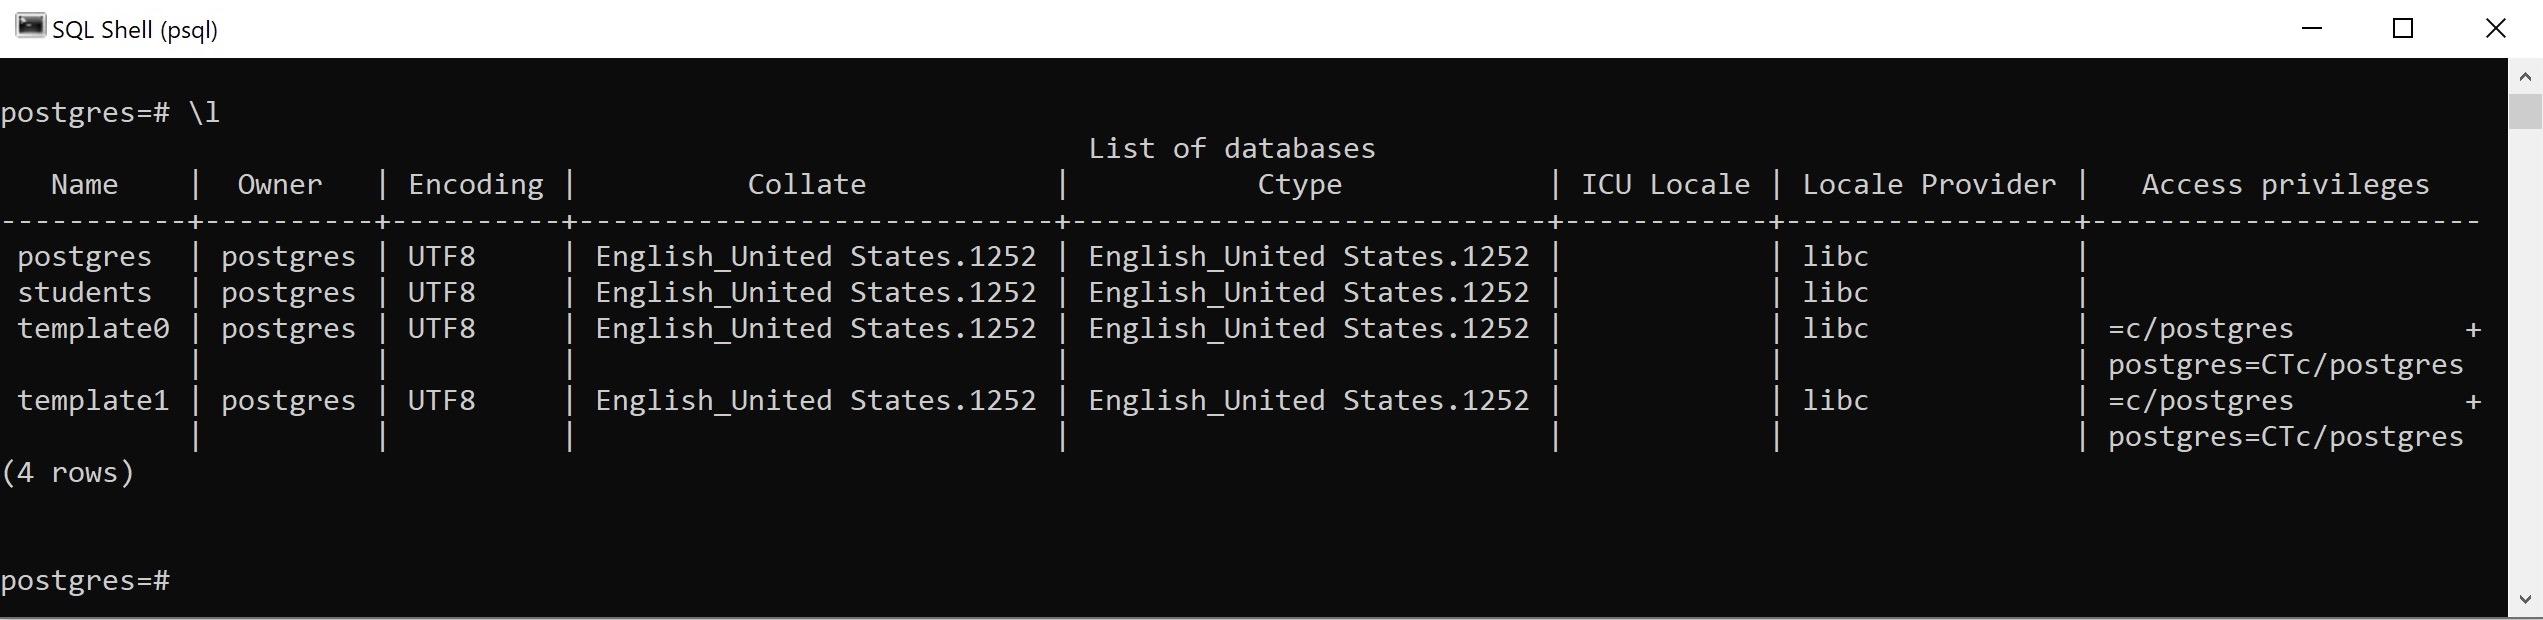
\includegraphics[width=.98\textwidth, trim={0cm 7cm 38cm 0cm},clip]{images/ch12/lstdbstu.jpg}};
    \drawshadow{image}
\end{tikzpicture}
\caption{}
\label{fig:lstdbstu}
\end{figure}



ဒေတာဘေ့စ်ထဲမှာ \fEn{table} တွေ ဆောက်ပါမယ်။ လက်ရှိအသုံးပြုမဲ့ ဒေတာဘေ့စ်နဲ့ \fEn{connection} အရင်ယူရမယ်။ \fEn{students} ဒေတာဘေ့စ်မှာ  \fEn{table} ဆောက်မှာ။ ဒီတော့ ချိတ်ဆက်မဲ့ \fCode{dbname} က \fCode{students} ဖြစ်တယ်။ ကျန်တာတွေက ရှေ့ကနဲ့ တူတူပဲ။
%
\begin{py}
import psycopg2

# Now, connect to the "students" database to create the "student" table
conn = psycopg2.connect(
    dbname="students",
    user="postgres",
    password="asdfgh",
    host="localhost",
    port="5432"
)
cur = conn.cursor()

# Create the "student" table
cur.execute("""
    CREATE TABLE student (
        id SERIAL PRIMARY KEY,
        name VARCHAR(100),
        age INT,
        grade VARCHAR(2)
    )
""")

# Commit changes and close the connection
conn.commit()
cur.close()
conn.close()
\end{py}
%

\fEn{Table} ဆောက်တဲ့ \fCode{CREATE TABLE} စတိတ်မန့်က  \fEn{auto-commit mode} \fEn{ON} ဖြစ်ဖြစ်၊ \fEn{OFF} ဖြစ်ဖြစ် \fEn{run} လို့ရတယ်။ \fEn{PostgreSQL} မှာ \fEn{default} က \fEn{OFF} ဖြစ်တယ်။ \fEn{Connection} ယူပြီးတာနဲ့ အခုလို တကူးတက ထည့်ပေးမယ်ဆိုရင်လည်း ပြဿနာတော့ မရှိပါဘူး။ 
%
\begin{py}
conn.autocommit = False
\end{py}
%
\fEn{Default} က \fEn{OFF} ဖြစ်ပြီးသားမို့လို့ လိုတော့မလိုအပ်ဘူး။

\fEn{Auto-commit} \fEn{OFF} ထားရင် \fEn{SQL} စတိတ်မန့် \fEn{execute} လုပ်ပြီး \fEn{commit} လုပ်ပေးဖို့ လိုတယ်။ ဒီအတွက်
%
\begin{py}
conn.commit()
\end{py}
%
လုပ်ရပါမယ်။ ဒါ မေ့ကျန်ခဲ့ရင် \fEn{execute} လုပ်ထားတဲ့ \fEn{SQL} က သက်ရောက်မှု ရှိမှာမဟုတ်ပါဘူး။ တစ်နည်းအားဖြင့် \fEn{student table} အမှန်တကယ် မဆောက်ပေးတော့ဘူး။ အကယ်၍ \fEn{auto-commit} \fEn{OFF} ထားရင်တော့ ကိုယ်တိုင် \fCode{conn.commit()} လုပ်မပေးရဘူး၊ ဒေတာဘေ့စ်က \fEn{SQL} ကွန်မန်း တစ်ခု \fEn{execute} လုပ်ပြီးတိုင်း အလိုအလျောက် \fEn{commit} လုပ်ပေးမှာပါ။ \fEn{OFF} ထားရင် \fCode{conn.commit()} လုပ်ပေးရမယ်၊ \fEn{ON} ဆိုရင် မလုပ်ပေးရဘူး၊ ဒီလို မှတ်ထားလို့ရတယ်။


